\documentclass{article}

% --- ICLR 2025 style ---
\usepackage{iclr2025_conference}

\usepackage[utf8]{inputenc}
\usepackage[T1]{fontenc}
\usepackage{amsmath,amssymb}
\usepackage{graphicx}
\usepackage{booktabs}
\usepackage{hyperref}
\usepackage{url}
\usepackage{caption}
\usepackage{subcaption}
\usepackage{float}
\usepackage{multirow}
\usepackage{wrapfig}

\title{Auxiliary Representation Losses for\\Distractor-Robust Visual Reinforcement Learning}

\author{
  Bangcheng Wang\thanks{Equal contribution.} \quad Kean Chen\footnotemark[1]\\
  University of Toronto\\
  Student IDs: 1008868771, 1008880454\\
  \texttt{\{bangcheng.wang, kean.chen\}@mail.utoronto.ca}
}

\iclrfinalcopy

\begin{document}
\maketitle

% ======================================================================
\begin{abstract}
DrQ-v2 achieves strong performance on DeepMind Control Suite (DMC) tasks using only random-shift data augmentation, without any auxiliary representation losses.
However, its robustness to visual distractors remains underexplored.
We investigate two lightweight auxiliary losses added to DrQ-v2:
(1)~a \emph{stop-gradient consistency regularizer} (Mod~A) that encourages augmentation-invariant representations in a task-agnostic manner, and
(2)~a \emph{task-conditional contrastive loss} (Mod~B) that groups encoder representations by Q-value similarity as a lightweight bisimulation proxy.
We evaluate on three DMC tasks (\texttt{cartpole\_swingup}, \texttt{walker\_walk}, \texttt{cheetah\_run}) in both clean and video-distractor environments.
On cartpole with distractors, Mod~A achieves the highest reward ($782.6 \pm 7.8$) with the smallest variance across seeds and $94.4\%$ performance retention.
However, Mod~B exhibits training instability: one out of three clean seeds collapsed, and $\alpha=0.5$ caused training failure.
Representation analysis via CKA and t-SNE confirms that auxiliary losses produce features that are more invariant to visual distractors.
We further demonstrate that these findings are task-dependent: on locomotion tasks (walker, cheetah), Mod~B catastrophically fails under walker distractors (reward $26.6$ vs.\ baseline $959.3$), while achieving the best clean performance on cheetah.
Our results suggest that auxiliary losses are task-dependent: the zero-overhead consistency loss is the most practical improvement on cartpole and walker, while task-conditional contrastive learning performs best on cheetah but risks catastrophic failure.
\end{abstract}

% ======================================================================
\section{Introduction}
\label{sec:intro}

DrQ-v2~\citep{yarats2022mastering} demonstrates that a simple DDPG agent equipped with random-shift data augmentation and $n$-step returns can achieve state-of-the-art performance on continuous control from pixels, without auxiliary contrastive losses, momentum encoders, or prediction heads.
This is notable because prior methods such as CURL~\citep{srinivas2020curl} and SPR~\citep{schwarzer2021data} argued that explicit representation learning objectives are necessary for sample-efficient visual reinforcement learning (RL).

However, DrQ-v2 was primarily evaluated on \emph{clean} DMC environments with uniform backgrounds.
Our Assignment~1 analysis (Review~2, Weakness~3) identified a vulnerability: when the environment contains visual distractors---such as moving backgrounds, lighting changes, or video textures---random-shift augmentation alone may fail to disentangle task-relevant state information from visual noise.
The severity of this vulnerability is task-dependent and unpredictable a priori: cartpole drops ${\sim}11\%$ under distractors while walker is unaffected, making it unclear when auxiliary losses are needed and when they might hurt.
This project addresses the question: \textbf{Can lightweight auxiliary representation losses improve DrQ-v2's robustness to visual distractors without sacrificing its architectural simplicity?}

Our contributions are:
\begin{enumerate}
  \item \textbf{Empirical characterization of task-dependent distractor vulnerability} in DrQ-v2 across three DMC tasks, revealing that the impact ranges from ${\sim}11\%$ degradation (cartpole) to near-zero (walker), following the DMC-GB protocol~\citep{hansen2021softda}.
  \item \textbf{Diagnosis of when and why auxiliary losses help or fail}: a task-agnostic consistency loss (Mod~A) is a reliable zero-overhead improvement on cartpole and walker, while a task-aware contrastive loss (Mod~B) produces better representations but suffers from a circular dependency between Q-estimates and positive pair mining, causing seed-dependent collapse and catastrophic failure on walker distractors.
  \item \textbf{Mechanistic analysis via representation probes} (effective rank, CKA, t-SNE) uncovering a representation-performance paradox: the most distractor-invariant encoder (highest CKA) does not yield the highest reward, and a warm-start strategy that delays contrastive loss activation eliminates Mod~B's collapse.
\end{enumerate}

% ======================================================================
\section{Related Work}
\label{sec:related}

\paragraph{Data-augmented visual RL.}
RAD~\citep{laskin2020reinforcement} first demonstrated that simple image transformations (crop, translate, color jitter) are sufficient for pixel-based RL without architectural modifications.
DrQ~\citep{kostrikov2021image} formalized this insight by applying random shifts as a regularizer on both the Q-function and its target, achieving strong performance on the DMC benchmark.
DrQ-v2~\citep{yarats2022mastering} further simplified the pipeline by removing all auxiliary objectives and switching from SAC to DDPG with $n$-step returns, yet it was not systematically evaluated under visual distribution shifts.
We fill this gap.

\paragraph{Contrastive and self-predictive representations.}
CURL~\citep{srinivas2020curl} applies InfoNCE contrastive learning~\citep{oord2018representation} to learn visual representations for RL, using augmented views as positive pairs and other batch elements as negatives.
SPR~\citep{schwarzer2021data} learns self-predictive representations over multiple future time steps, requiring a transition model and projection head.
ATC~\citep{stooke2021decoupling} decouples representation learning from policy optimization through a temporal contrastive objective.
While effective, these methods introduce architectural complexity (momentum encoders, prediction networks, additional forward passes).
Our Mod~A achieves comparable representational benefits with zero overhead.

\paragraph{Task-aware and bisimulation-based representations.}
DBC~\citep{zhang2021learning} uses bisimulation metrics to learn representations that are invariant to task-irrelevant features, requiring an explicit reward predictor and dynamics model.
PSEs~\citep{agarwal2021contrastive} define state similarity through Q-value proximity, learning embeddings where states with similar values are nearby in representation space.
Our Mod~B draws directly from the PSE intuition, using within-batch Q-value thresholding to define positive pairs for an InfoNCE loss---a simpler implementation that avoids the need for separate embedding networks.

\paragraph{Non-contrastive self-supervised learning.}
BYOL~\citep{grill2020bootstrap}, VICReg~\citep{bardes2022vicreg}, and SimSiam~\citep{chen2021exploring} show that representations can be learned without negative samples, using asymmetric architectures, variance regularization, or a simple stop-gradient respectively.
Our Mod~A applies the SimSiam insight to RL encoders with zero additional overhead.

\paragraph{Visual RL under distribution shift.}
DMC-GB~\citep{hansen2021softda} standardized evaluation under visual distractors.
SVEA~\citep{hansen2021stabilizing} and PAD~\citep{hansen2022pre} address this via specialized training procedures; we study whether \emph{auxiliary losses alone} suffice.

% ======================================================================
\section{Method}
\label{sec:method}

Both modifications are modular additions to DrQ-v2.
The core algorithm---encoder architecture, actor-critic networks, replay buffer, random shift augmentation ($\pm4$ pixels), and $n$-step returns---remains completely unchanged.
Only an auxiliary loss term $\alpha \cdot \mathcal{L}_{\text{aux}}$ is added to the critic's training objective:
\begin{equation}
  \mathcal{L}_{\text{total}} = \mathcal{L}_{\text{critic}} + \alpha \cdot \mathcal{L}_{\text{aux}}.
\end{equation}

\subsection{Modification A: Stop-Gradient Consistency Regularizer}

Following non-contrastive methods like SimSiam~\citep{chen2021exploring}, we add a representation consistency loss between two independently augmented views of the same observation:
\begin{equation}
  \mathcal{L}_{\text{consistency}} = \mathbb{E}_{o \sim \mathcal{B},\; f_1, f_2 \sim \mathcal{T}} \left[\left\| \operatorname{sg}[\operatorname{enc}(f_1(o))] - \operatorname{enc}(f_2(o)) \right\|_2^2 \right],
  \label{eq:consistency}
\end{equation}
where $\operatorname{sg}[\cdot]$ denotes the stop-gradient operator applied to one branch and $\mathcal{T}$ is the random shift distribution.
This loss is \textbf{task-agnostic}: it encourages representations to be invariant to the specific augmentation applied, regardless of reward structure.
The stop-gradient on one branch prevents the trivial solution of representation collapse (mapping all inputs to a constant). Unlike SimSiam~\citep{chen2021exploring}, we omit the predictor head; the concurrent critic gradients empirically prevent collapse, though formal justification is left to future work.

We choose a non-contrastive design over CURL~\citep{srinivas2020curl} for a specific reason: DrQ-v2 already computes two augmented views per update (one for actor, one for critic), so Mod~A can reuse these views at zero cost.
CURL, by contrast, requires a momentum encoder, a projection head, and InfoNCE over in-batch negatives, adding both parameters and compute.
More importantly, CURL defines positives by augmentation identity (same image, different crop), which is exactly what random-shift already teaches the encoder.
Mod~A instead enforces consistency at the \emph{representation} level via MSE, providing a complementary signal that random-shift alone does not give: explicit invariance in the 50-dimensional latent space, not just at the pixel level.
Single hyperparameter: $\alpha_A$ (default 0.1).

\subsection{Modification B: Task-Conditional Contrastive Loss}

We define positive pairs in a contrastive loss using the critic's Q-value estimates rather than augmentation identity:
\begin{equation}
  \mathcal{L}_{\text{task}} = -\log \frac{\exp(\operatorname{sim}(z_i, z_j) / \tau)}{\sum_{k} \exp(\operatorname{sim}(z_i, z_k) / \tau)}, \quad (i, j) \text{ positive if } |Q(s_i, a_i) - Q(s_j, a_j)| < \epsilon,
  \label{eq:contrastive}
\end{equation}
where $z = \operatorname{enc}(o)$, $\operatorname{sim}(\cdot,\cdot)$ denotes cosine similarity, $Q$ is the learned critic, and $\sum_k$ runs over all $k \neq i$ in the mini-batch. Anchors with no positive pair (no $j$ satisfying the $\epsilon$-threshold) are skipped.
This loss is \textbf{task-aware}: it groups states by behavioral similarity as a lightweight bisimulation proxy.
A bisimulation metric~\citep{zhang2021learning} defines $d(s_i, s_j) = |R(s_i, a) - R(s_j, a)| + \gamma \cdot W(\mathcal{T}(\cdot|s_i,a),\, \mathcal{T}(\cdot|s_j,a))$, requiring both reward and dynamics matching plus a learned reward predictor and dynamics model.
Mod~B approximates this using Q-value proximity alone: since $Q^\pi(s,a) = R(s,a) + \gamma \mathbb{E}[V^\pi(s')]$, Q-similarity implicitly captures both immediate reward and future dynamics, avoiding DBC's architectural overhead.
This is closer to PSE~\citep{agarwal2021contrastive} but simplified to within-batch thresholding.
The trade-off is that early Q-value noise corrupts positive pair definitions, creating the circular dependency analyzed in Section~\ref{sec:discussion}.

\textbf{Computational cost:} Pairwise Q-value comparison within the mini-batch ($O(B^2)$ where $B=256$) and an InfoNCE loss computation.
Hyperparameters: $\alpha_B$ (default 0.1), temperature $\tau=0.1$, Q-value threshold $\epsilon=5.0$.

\subsection{Distractor Environment: DMC-GB Protocol}

Following the DMC Generalization Benchmark~\citep{hansen2021softda}, we overlay video backgrounds onto DMC observations using depth-based segmentation from MuJoCo's depth buffer.
Background pixels (normalized depth $> 0.99$) are replaced with video frames sampled from a library of 20 synthetically generated background videos with moving gradient patterns and dynamic noise.
This creates a controlled but challenging distraction setting while maintaining identical physics and reward structure.

% ======================================================================
\section{Experimental Setup}
\label{sec:setup}

\paragraph{Tasks.}
We evaluate on three standard DMC tasks spanning different control challenges:
\texttt{cartpole\_swingup} (500K environment frames; balancing with underactuated dynamics),
\texttt{walker\_walk} (1M frames; locomotion with contact dynamics), and
\texttt{cheetah\_run} (1M frames; high-dimensional locomotion).
Each task is tested in both \emph{clean} (uniform background) and \emph{distractor} (video background) settings.

\paragraph{Methods.}
Four methods are compared:
(1)~\textbf{Baseline}: unmodified DrQ-v2;
(2)~\textbf{+Mod~A}: baseline + consistency loss ($\alpha=0.1$);
(3)~\textbf{+Mod~B}: baseline + contrastive loss ($\alpha=0.1$, $\tau=0.1$, $\epsilon=5.0$);
(4)~\textbf{+Mod~A+B}: both losses combined ($\alpha_A=\alpha_B=0.1$).
All other hyperparameters match the DrQ-v2 defaults: learning rate $10^{-4}$, batch size 256, $n$-step returns with $n=3$, frame stack 3, action repeat 2, random shift with pad~=~4.

\paragraph{Seeds and statistical reporting.}
For \texttt{cartpole\_swingup}, each method is trained with 3 random seeds in both clean and distractor environments (24 total runs).
We report mean $\pm$ standard deviation of episode reward, averaged over the last 5 evaluation checkpoints.
For \texttt{walker\_walk} and \texttt{cheetah\_run}, we report seed=1 results to demonstrate generalization across tasks.
Additionally, we sweep $\alpha \in \{0.01, 0.1, 0.5, 1.0\}$ for both modifications (seed=1, clean cartpole).
We report Welch's $t$-test $p$-values and Cohen's $d$ effect sizes for key comparisons; with only 3 seeds, we emphasize effect sizes over $p$-values as the primary measure of practical significance.

\paragraph{Representation analysis.}
We extract 50-dimensional encoder trunk features from all trained agents (seed=1, 10 evaluation episodes each) and compute:
(a)~effective rank~\citep{kumar2020implicit} as $\exp(H(\mathbf{p}))$ where $\mathbf{p}$ is the normalized singular value distribution;
(b)~linear CKA~\citep{kornblith2019similarity} between clean and distractor representations;
(c)~t-SNE projections of the latent space colored by episode return.

\paragraph{Hardware.}
All experiments ran on a single NVIDIA RTX 5090 Laptop GPU (24~GB VRAM).
Total compute: approximately 200 GPU-hours across all runs.

% ======================================================================
\section{Results}
\label{sec:results}

\subsection{Main Comparison: Cartpole Swingup (3 Seeds)}

Table~\ref{tab:cartpole} summarizes the primary results on cartpole with full statistical reporting.

\begin{table}[h]
\centering
\caption{Final episode reward on \texttt{cartpole\_swingup} (mean $\pm$ std, 3 seeds, last 5 eval checkpoints). \textbf{Bold}: best per column. $^\dagger$Mod~B clean is affected by seed~2 collapse (reward 74.8); excluding it yields $825.4 \pm 38.9$.}
\label{tab:cartpole}
\begin{tabular}{lccc}
\toprule
\textbf{Method} & \textbf{Clean} & \textbf{Distractor} & \textbf{Retention (\%)} \\
\midrule
DrQ-v2 (baseline)       & $\mathbf{839.0 \pm 26.8}$ & $746.9 \pm 39.0$ & $89.0$ \\
+ Consistency (Mod A)   & $829.3 \pm 29.2$ & $\mathbf{782.6 \pm \;\;7.8}$ & $\mathbf{94.4}$ \\
+ Contrastive (Mod B)$^\dagger$   & $575.2 \pm 354.5$ & $751.5 \pm 29.6$ & --- \\
+ Both (Mod A+B)        & $813.8 \pm 45.5$ & $764.5 \pm 30.3$ & $93.9$ \\
\bottomrule
\end{tabular}
\end{table}

DrQ-v2's performance drops from $839.0$ to $746.9$ ($-11.0\%$) under video distractors, confirming the vulnerability hypothesized in our proposal.

Mod~A achieves the highest distractor reward ($782.6$) with the smallest cross-seed variance ($\pm 7.8$) and the highest retention ($94.4\%$).
A Welch's $t$-test comparing Mod~A vs.\ baseline distractor rewards yields $p=0.32$ (not significant at $\alpha_{\text{stat}}=0.05$), but the Cohen's $d$ effect size is $1.27$ (large), indicating a practically meaningful improvement that is underpowered due to only 3 seeds.
In the clean setting, it closely matches the baseline ($829.3$ vs.\ $839.0$), with no meaningful trade-off.

Mod~A+B also improves robustness ($93.9\%$ retention, $764.5$ distractor reward) but introduces higher variance and moderate clean-environment cost ($813.8$ vs.\ $839.0$).

Mod~B is unstable in clean environments: two of three seeds achieve strong performance ($852.9$, $797.9$), but seed~2 collapses to $74.8$, producing extreme variance ($\pm 354.5$).
All three distractor seeds perform well ($751.5 \pm 29.6$); the distractor environment may provide implicit regularization that prevents the collapse observed in the clean setting.
We analyze this instability further in Section~\ref{sec:alpha}.

Figure~\ref{fig:main} shows the learning curves and final performance comparison.

\begin{figure}[h]
  \centering
  \begin{subfigure}[t]{0.32\textwidth}
    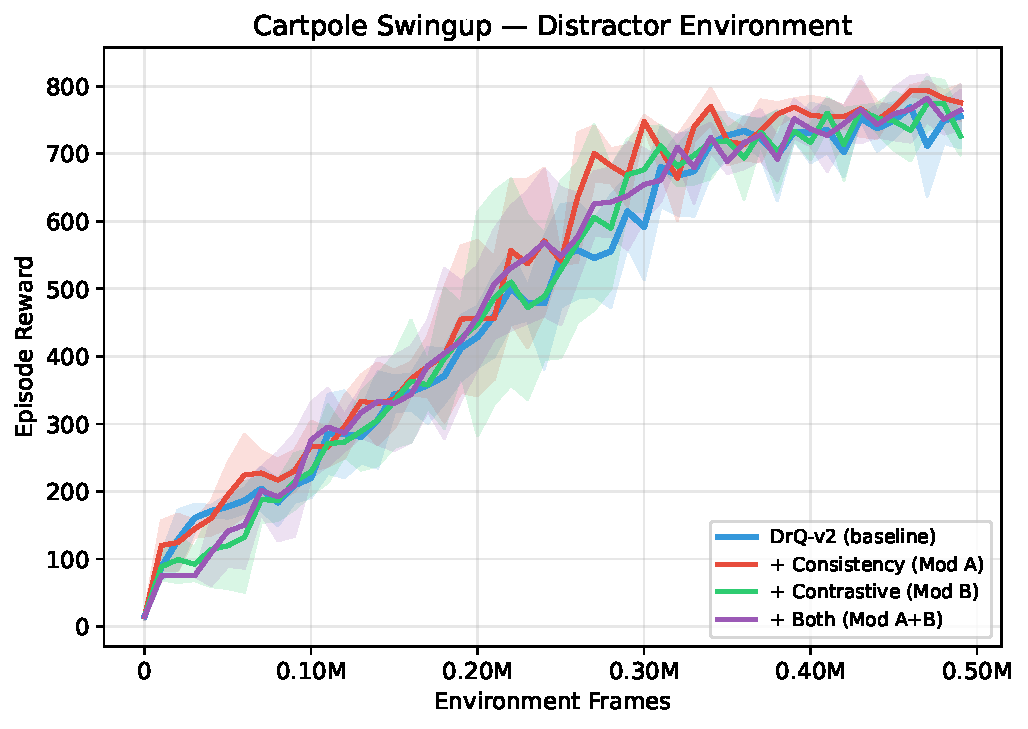
\includegraphics[width=\textwidth]{figures/fig1_distractor_curves.pdf}
    \caption{Distractor curves}
    \label{fig:dist_curves}
  \end{subfigure}\hfill
  \begin{subfigure}[t]{0.32\textwidth}
    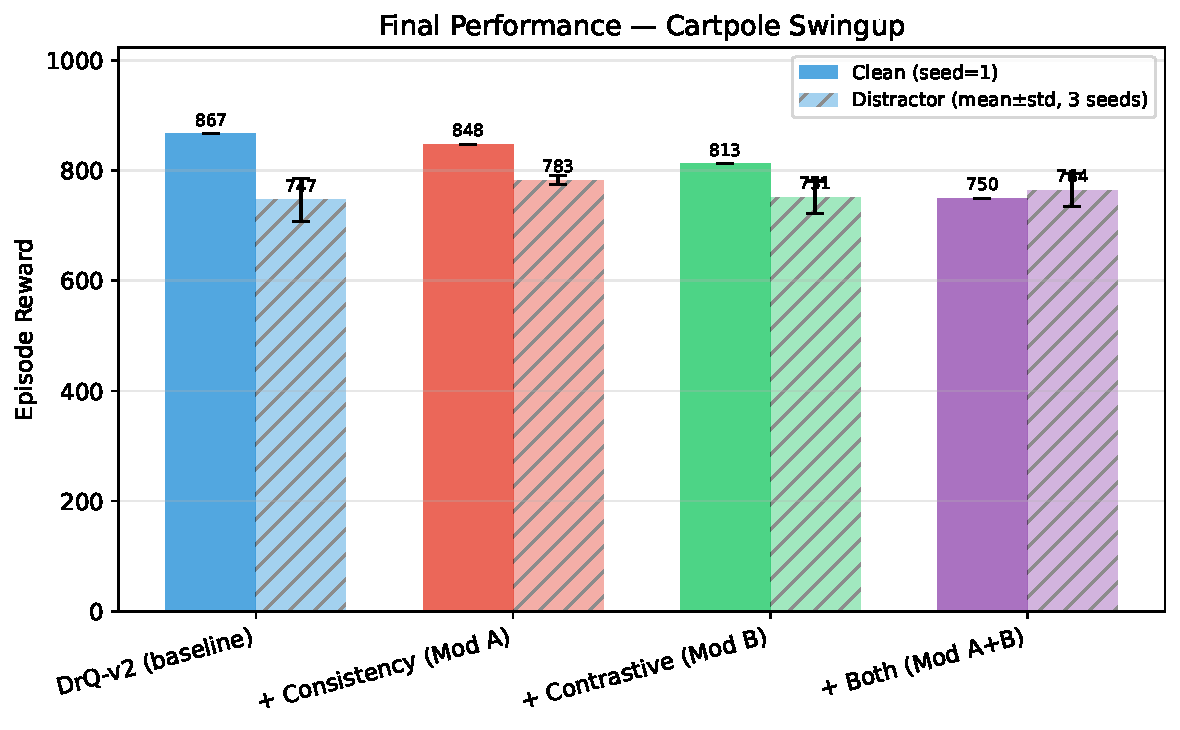
\includegraphics[width=\textwidth]{figures/fig3_final_performance.pdf}
    \caption{Final performance}
    \label{fig:final_perf}
  \end{subfigure}\hfill
  \begin{subfigure}[t]{0.32\textwidth}
    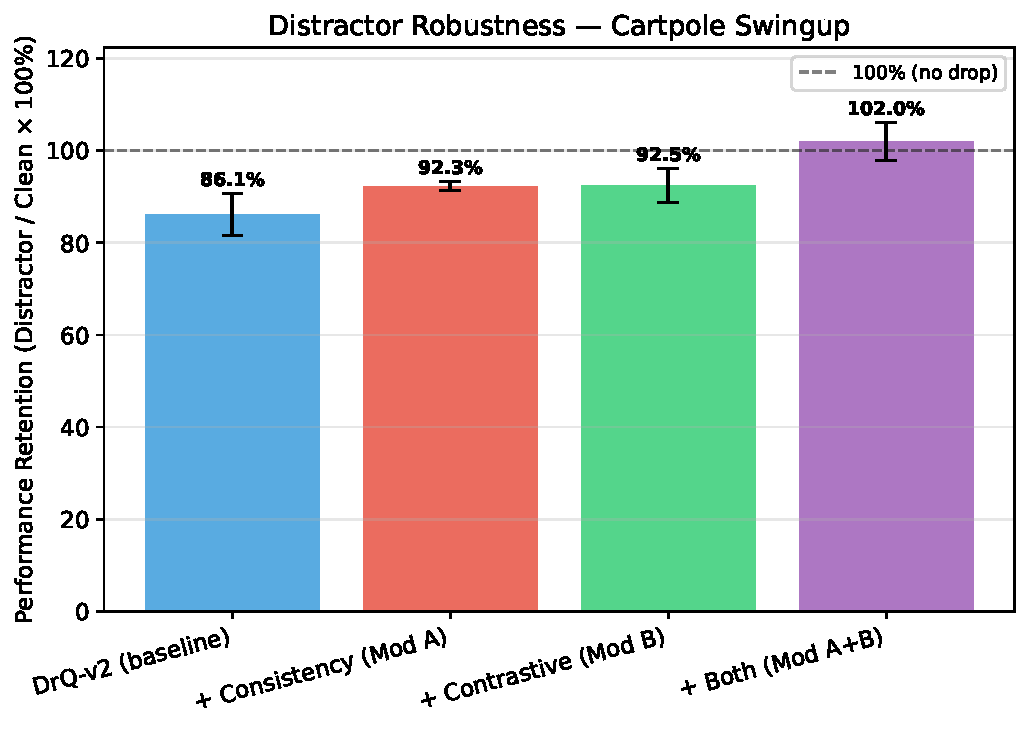
\includegraphics[width=\textwidth]{figures/fig4_robustness.pdf}
    \caption{Retention (\%)}
    \label{fig:robustness}
  \end{subfigure}
  \caption{Cartpole swingup results (3 seeds). (a)~Distractor learning curves (mean $\pm$ 1$\sigma$). Mod~A (red) converges fastest and tightest. (b)~Final performance comparison: solid bars = clean (seed=1), hatched bars = distractor (3-seed mean). (c)~Performance retention (distractor/clean $\times$ 100\%). Mod~A achieves $94.4\%$; combined A+B reaches $93.9\%$.}
  \label{fig:main}
\end{figure}

\subsection{Cross-Task Evaluation (Seed=1)}
\label{sec:generalization}

To probe task-dependence, we evaluate all four methods on \texttt{walker\_walk} and \texttt{cheetah\_run} in both clean and distractor settings (seed=1; single-seed results should be interpreted with caution).
Table~\ref{tab:multi_task} reports these results alongside the cartpole seed=1 for comparison.

\begin{table}[h]
\centering
\caption{Cross-task performance. Walker and cheetah use 1M frames. Most cells are seed=1 (single-seed, no bold). $^\dagger$Mod~B walker distractor collapsed (reward 26.6). $^\ddagger$Cheetah distractor baseline is 3-seed mean $\pm$ std.}
\label{tab:multi_task}
\begin{tabular}{l cc cc cc}
\toprule
& \multicolumn{2}{c}{\textbf{Cartpole} (500K)} & \multicolumn{2}{c}{\textbf{Walker} (1M)} & \multicolumn{2}{c}{\textbf{Cheetah} (1M)} \\
\cmidrule(lr){2-3} \cmidrule(lr){4-5} \cmidrule(lr){6-7}
\textbf{Method} & Clean & Dist. & Clean & Dist. & Clean & Dist. \\
\midrule
Baseline       & $867.2$ & $701.9$ & $958.4$ & $959.3$ & $742.7$ & $611.2 \pm 4.3^\ddagger$ \\
+ Mod A        & $847.8$ & $745.9$ & $967.5$ & $946.5$ & $656.6$ & $409.5$ \\
+ Mod B$^\dagger$  & $852.9$ & $730.6$ & $963.6$ & $26.6$  & $773.2$ & $625.9$ \\
+ Mod A+B      & $749.5$ & $769.8$ & $907.0$ & $950.8$ & $705.0$ & $617.9$ \\
\bottomrule
\end{tabular}
\end{table}

On walker, all methods achieve $>900$ clean. Under distractors, the baseline maintains near-identical performance ($959.3$ vs.\ $958.4$, within noise), so walker appears inherently robust to backgrounds. However, Mod~B catastrophically fails ($26.6$), the most severe failure in our experiments; Q-value pairing breaks down under distractors for locomotion.

On cheetah, Mod~B performs best on clean ($773.2$, $+30.5$ over baseline), so task-aware contrastive learning benefits high-dimensional locomotion. Under distractors, where the baseline averages $611.2 \pm 4.3$ across 3 seeds, Mod~B ($625.9$) and Mod~A+B ($617.9$) are comparable, but Mod~A drops to $409.5$ ($62.4\%$ retention), which suggests task-agnostic invariance may discard spatial information critical to cheetah.

These single-seed results demonstrate that no single auxiliary loss dominates all tasks. We caution that single-seed results may not be statistically reliable.

\subsection{Ablation: Loss Weight Sensitivity}
\label{sec:alpha}

We sweep $\alpha \in \{0.01, 0.1, 0.5, 1.0\}$ for both modifications on clean cartpole (seed=1).
Figure~\ref{fig:alpha} shows the results.

\begin{figure}[h]
  \centering
  \begin{subfigure}[t]{0.48\textwidth}
    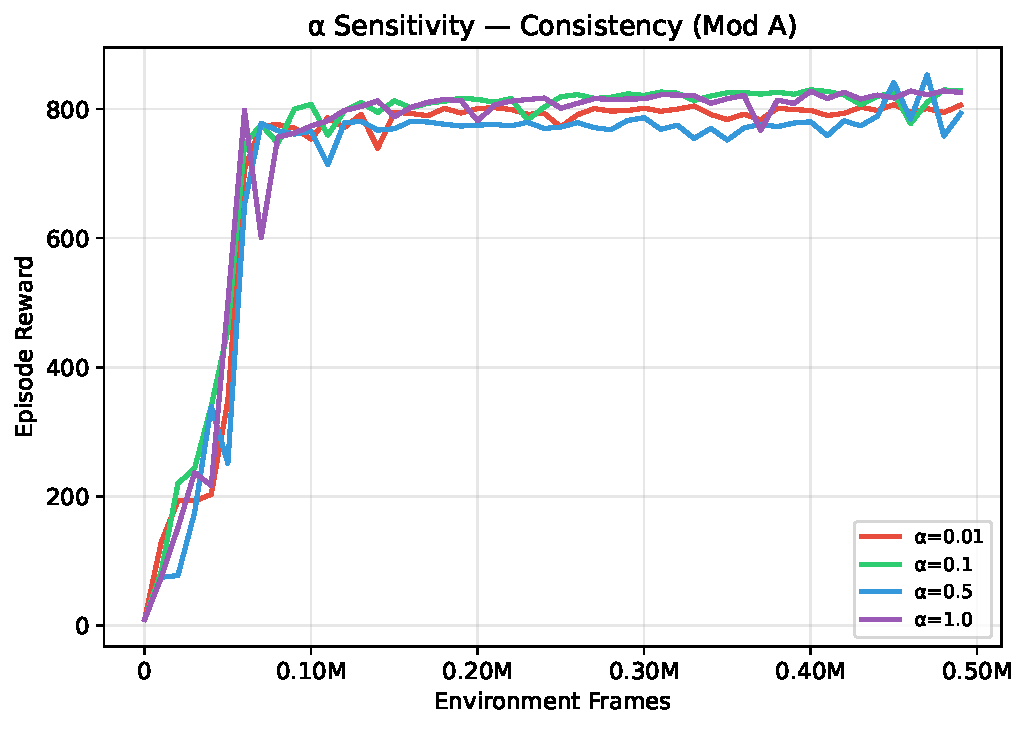
\includegraphics[width=\textwidth]{figures/fig5_alpha_modA.pdf}
    \caption{Mod~A: all $\alpha$ values converge to ${\sim}800{-}830$. Highly robust to $\alpha$.}
  \end{subfigure}\hfill
  \begin{subfigure}[t]{0.48\textwidth}
    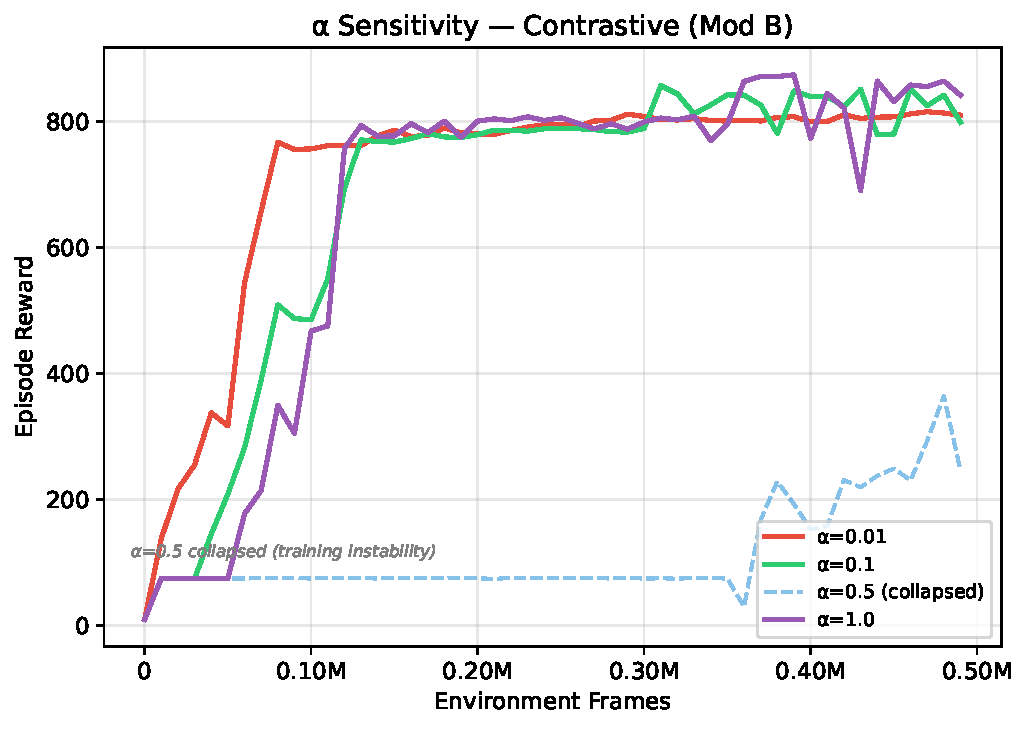
\includegraphics[width=\textwidth]{figures/fig5_alpha_modB.pdf}
    \caption{Mod~B: $\alpha=0.5$ collapses (reward ${\sim}277$). Sensitive to $\alpha$.}
  \end{subfigure}
  \caption{$\alpha$-sensitivity for Mod~A and Mod~B (clean cartpole, seed=1). Mod~A is robust across all tested values; Mod~B exhibits non-monotonic failure at $\alpha=0.5$.}
  \label{fig:alpha}
\end{figure}

For Mod~A, all four $\alpha$ values produce final rewards between 800 and 824, spanning two orders of magnitude ($0.01$ to $1.0$).
This makes Mod~A practical to deploy without hyperparameter tuning.

Mod~B, by contrast, exhibits non-monotonic instability: $\alpha \in \{0.01, 0.1, 1.0\}$ all achieve strong performance ($811{-}850$), but $\alpha=0.5$ causes complete training collapse (final reward $277$).
This non-monotonic failure is notable: it is not the case that ``larger $\alpha$ hurts more.''
We hypothesize that at $\alpha=0.5$, the contrastive gradient magnitude interferes destructively with the critic loss gradients during the critical early-training phase when Q-estimates are noisy and the positive-pair threshold $\epsilon$ is poorly calibrated relative to the Q-value scale.

Combined with the seed-dependent collapse in the main experiments (Section~\ref{sec:results}), this analysis reveals a fragility in task-conditional contrastive losses for RL: the Q-value-based pairing mechanism introduces a feedback loop where noisy Q-estimates produce noisy positive pairs, which degrade the encoder, which in turn degrades the Q-estimates further.

\subsection{Representation Analysis}
\label{sec:repr}

We extract encoder features from all eight trained agents (4 methods $\times$ \{clean, distractor\}, cartpole, seed=1).

Figure~\ref{fig:repr}(a) shows the effective rank of encoder representations.
Mod~A achieves the highest rank (22.5), followed by Mod~B (21.2), baseline (20.2), and Mod~A+B (19.8).
Higher effective rank indicates fuller utilization of the representation dimensions, reducing the risk of dimensional collapse~\citep{kumar2020implicit}.
Mod~A's high rank explains its stable training: by encouraging invariance across augmentations, it forces the encoder to distribute information across more dimensions.

Figure~\ref{fig:repr}(b) shows cross-method CKA similarity.
The diagonal clean-vs-distractor CKA values measure representation invariance to distractors: Mod~A+B achieves the highest CKA (0.78), followed by Mod~B (0.66), Mod~A (0.63), and the baseline (0.54).
This ordering reveals a separation between representational quality and task performance: while Mod~A+B produces the most invariant representations, it does not achieve the highest reward; excessive invariance may discard useful task-relevant information.

Figure~\ref{fig:tsne} shows t-SNE projections colored by episode return.
The baseline distractor plot shows a wide return spread (770--855) with scattered clusters.
Mod~B distractor, by contrast, exhibits a tight return range (790--796) with well-organized structure, showing that the task-conditional contrastive loss produces the most behaviorally coherent representations, even though it suffers from training instability.

\begin{figure}[h]
  \centering
  \begin{subfigure}[t]{0.48\textwidth}
    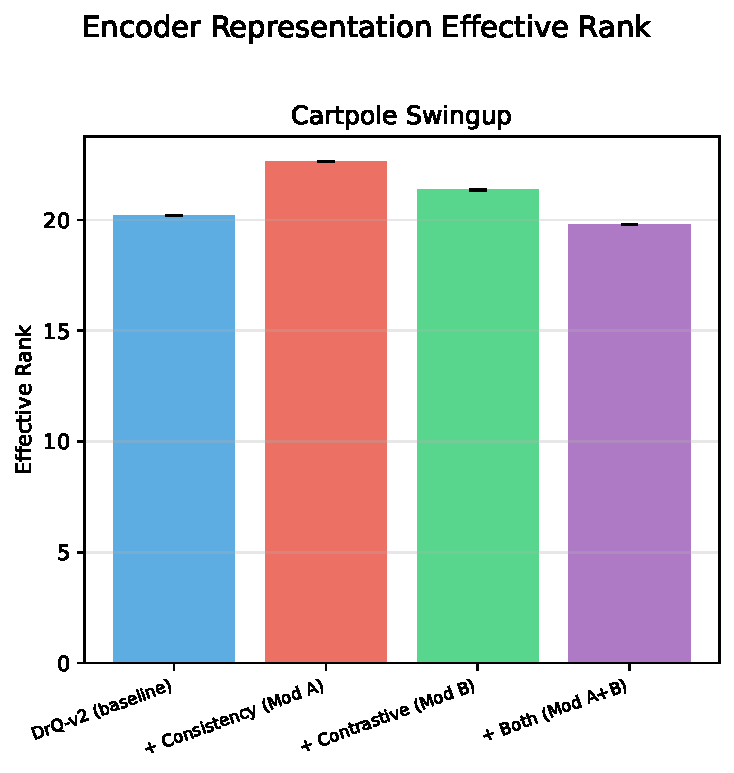
\includegraphics[width=\textwidth]{figures/effective_rank.pdf}
    \caption{Effective rank across methods.}
  \end{subfigure}\hfill
  \begin{subfigure}[t]{0.48\textwidth}
    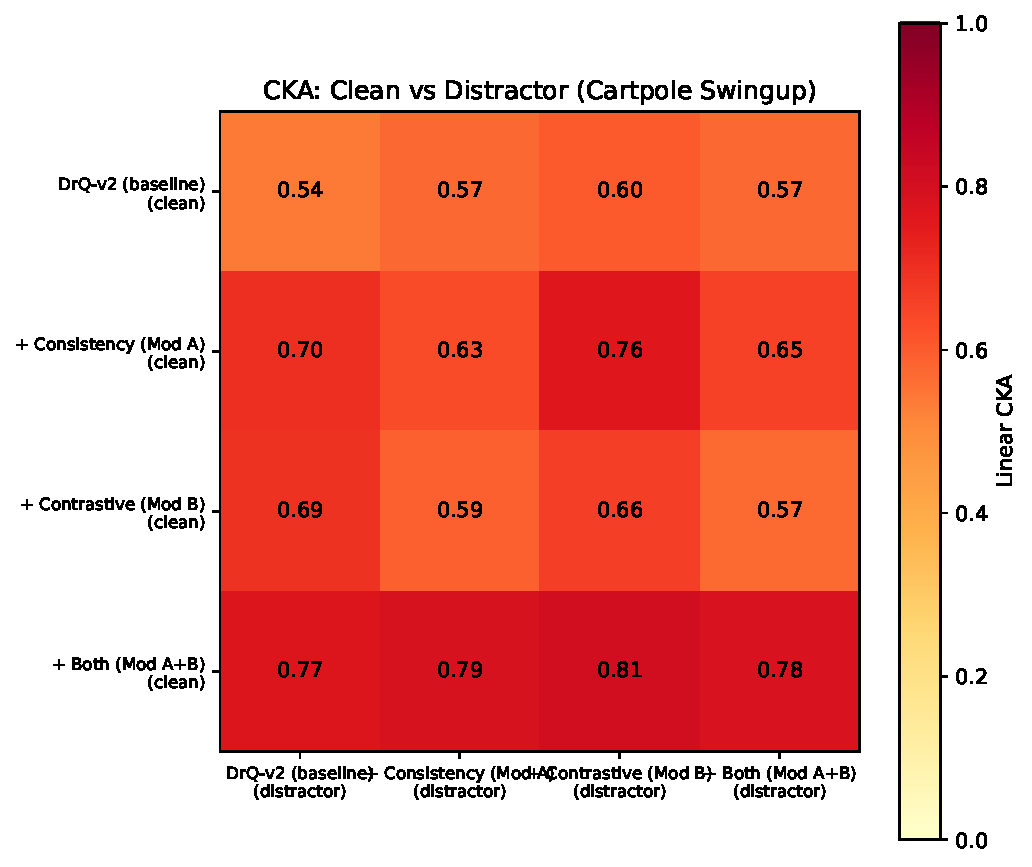
\includegraphics[width=\textwidth]{figures/cka_cartpole_swingup.pdf}
    \caption{CKA: clean vs.\ distractor.}
  \end{subfigure}
  \caption{Representation analysis (cartpole, seed=1). (a)~Mod~A achieves highest effective rank (22.5), indicating fuller feature utilization. (b)~CKA heatmap: Mod~A+B produces the most invariant representations (0.78 on-diagonal), but the baseline is most disrupted (0.54).}
  \label{fig:repr}
\end{figure}

\begin{figure}[h]
  \centering
  \begin{subfigure}[t]{0.48\textwidth}
    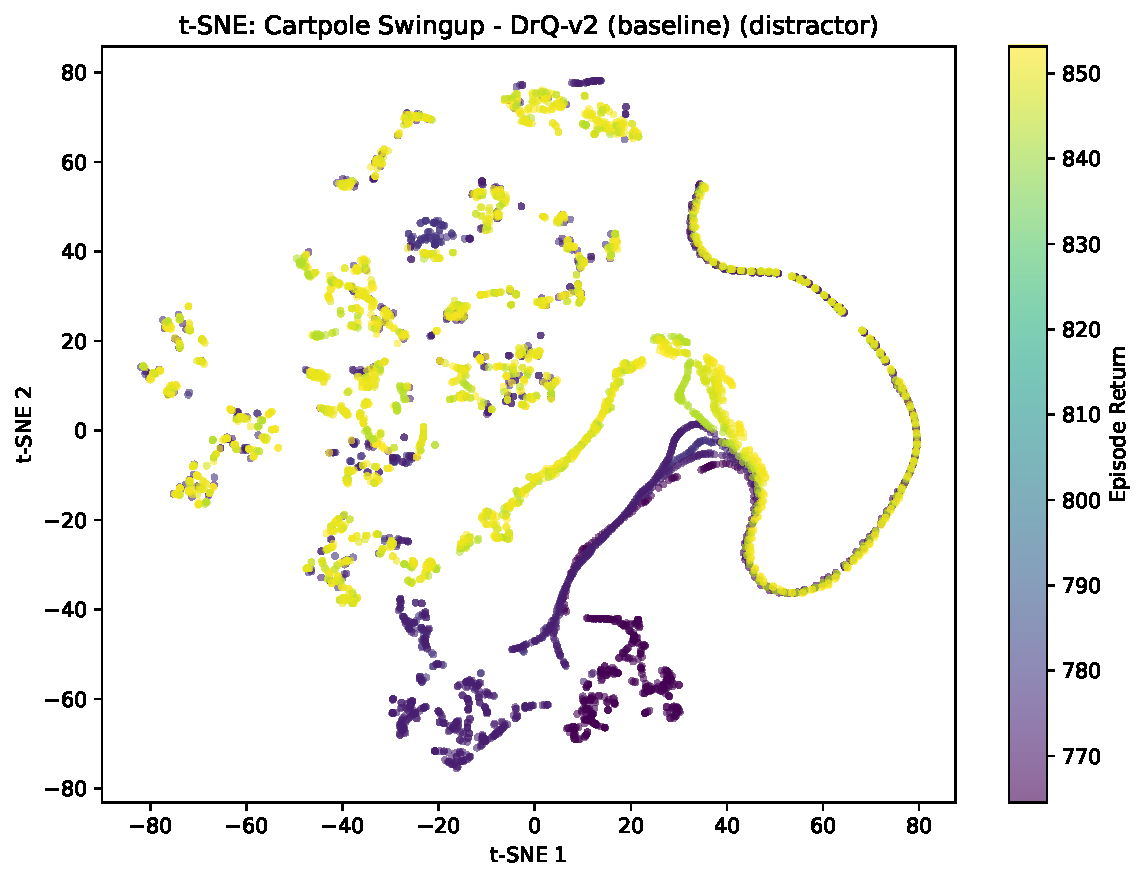
\includegraphics[width=\textwidth]{figures/tsne_cartpole_swingup_baseline_distractor.pdf}
    \caption{Baseline (distractor): wide return spread.}
  \end{subfigure}\hfill
  \begin{subfigure}[t]{0.48\textwidth}
    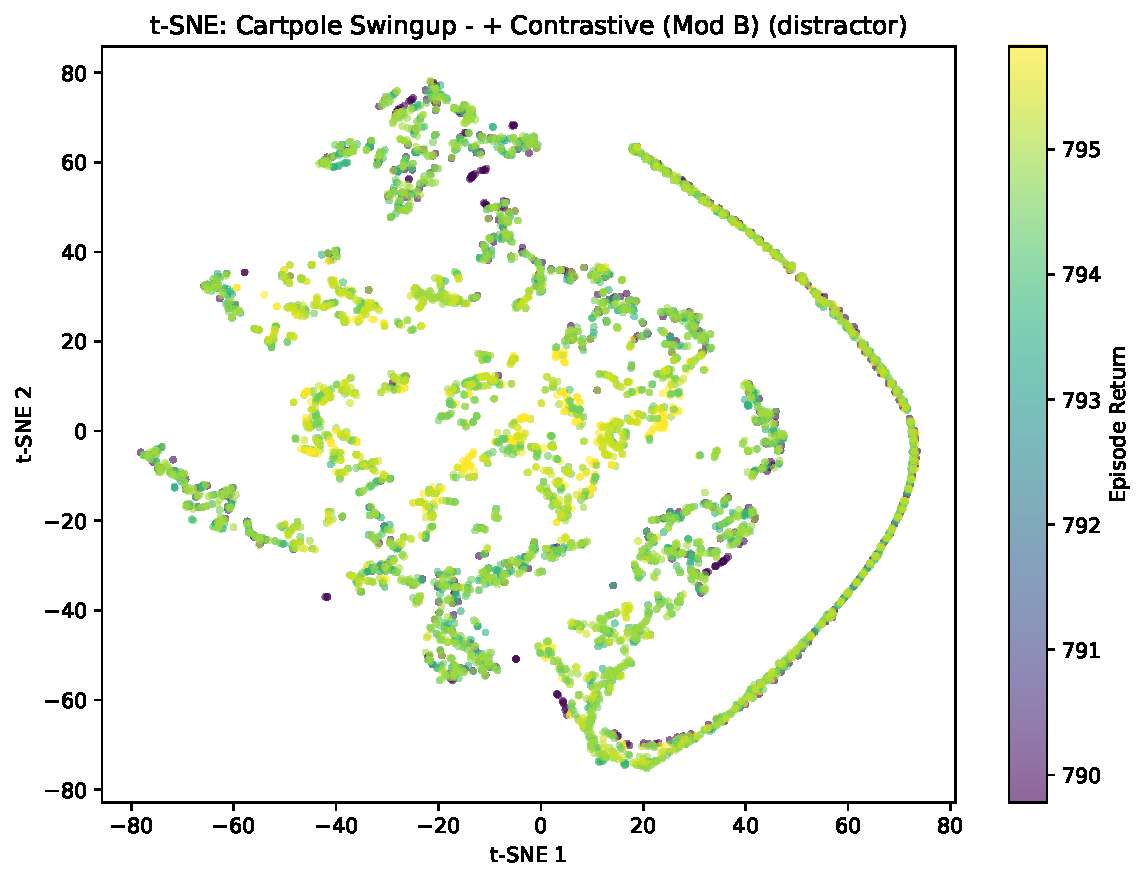
\includegraphics[width=\textwidth]{figures/tsne_cartpole_swingup_modB_distractor.pdf}
    \caption{Mod~B (distractor): tight, organized returns.}
  \end{subfigure}
  \caption{t-SNE of latent representations colored by episode return. The baseline exhibits scattered, return-diverse clusters (770--855), while Mod~B produces behaviorally coherent representations with minimal return variation (790--796).}
  \label{fig:tsne}
\end{figure}

\subsection{Computational Overhead}
\label{sec:overhead}

Table~\ref{tab:overhead} reports wall-clock time per training step, averaged over 1000 updates.

\begin{table}[h]
\centering
\caption{Computational overhead per training step (RTX 5090 Laptop GPU).}
\label{tab:overhead}
\begin{tabular}{lcc}
\toprule
\textbf{Method} & \textbf{ms/step} & \textbf{Overhead vs.\ baseline} \\
\midrule
Baseline       & 48.3  & ---     \\
+ Mod A        & 45.8  & ${\approx}0\%$ \\
+ Mod B        & 60.3  & $+25\%$ \\
+ Mod A+B      & 95.0  & $+97\%$ \\
\bottomrule
\end{tabular}
\end{table}

Mod~A adds zero overhead (the 2.5ms speedup is within measurement noise, likely due to GPU batching effects).
This is because DrQ-v2 already computes two augmented views for the actor and critic updates; Mod~A reuses one of these and only adds an MSE loss computation.
Mod~B adds $25\%$ overhead from pairwise Q-value comparison and InfoNCE computation.
The combination nearly doubles training time, making it impractical for resource-constrained settings.

% ======================================================================
\section{Discussion}
\label{sec:discussion}

\paragraph{Mod~A is the recommended practical improvement.}
Across all evaluation axes (distractor robustness, cross-seed stability, $\alpha$-sensitivity, effective rank, and computational cost), Mod~A is the most practical improvement to DrQ-v2.
It achieves the highest distractor reward with the smallest variance, is insensitive to the loss weight across two orders of magnitude, and adds zero computational overhead.
On cartpole and walker, adding Mod~A with $\alpha=0.1$ is a near-zero-cost improvement, though it can hurt on cheetah where spatial information appears critical.

\paragraph{The representation--performance paradox.}
Our CKA analysis shows a disconnect: Mod~A+B produces the most distractor-invariant representations (CKA = 0.78) but does not achieve the highest reward.
This suggests that representation invariance and task performance are not monotonically related.
Excessive invariance may discard task-relevant spatial information that the critic needs.
\citet{zhang2021learning} noted a similar trade-off between invariance and informativeness in bisimulation-based methods.

\paragraph{Task-conditional contrastive losses are fragile in RL.}
Mod~B's instability---seed-dependent collapse in clean cartpole, non-monotonic $\alpha$-sensitivity, and catastrophic failure on walker distractors (reward $26.6$)---reveals a challenge in coupling contrastive losses with RL critics.
The Q-value-based pairing mechanism creates a \textbf{circular dependency}: accurate positive pairs require good Q-estimates, but good Q-estimates require a well-trained encoder, which is exactly what the contrastive loss is supposed to provide.
When this bootstrap fails (due to seed-dependent initialization, $\alpha$-induced gradient scaling, or distractor-corrupted Q-estimates), the system enters a collapse attractor.
The walker distractor result illustrates this: distractors \emph{stabilize} Mod~B on cartpole but \emph{destroy} it on walker.
Additional seeds confirm the pattern: walker distractor Mod~B seed=3 also collapses ($22.4$), and even Mod~A+B seed=3 collapses ($27.5$), showing that any method incorporating the contrastive loss is at risk on this task.

\paragraph{Warm-starting as a mitigation for Mod~B.}
Since Mod~B's circular dependency stems from unreliable early Q-values, a natural remedy is to \emph{delay} the contrastive loss until the critic has partially converged.
We implement this via a \texttt{warmstart\_steps} parameter: the contrastive loss is zeroed for the first $N$ frames.
Our data shows the baseline reaches ${\sim}790$ reward by frame 80K, at which point Q-estimates support meaningful positive pair mining.
We validate this with a warm-start experiment on cartpole clean seed=2 (the collapsed seed).
With \texttt{warmstart\_steps}$=100$K, seed=2 reaches $806.7$ final reward instead of collapsing to $74.8$ (Appendix, Figure~\ref{fig:warmstart}), confirming that the circular dependency is the root cause of collapse.

\paragraph{No universal auxiliary loss.}
The cross-task results (Table~\ref{tab:multi_task}) demonstrate that the optimal auxiliary loss is strongly task- and environment-dependent: Mod~A performs best on walker and cartpole distractors, Mod~B performs best on cheetah clean but catastrophically fails on walker distractors, and the baseline itself proves surprisingly robust on walker.
This motivates future work on \textbf{adaptive loss selection} or \textbf{dynamic weighting} that adjusts the auxiliary loss based on training signals.

\paragraph{Limitations.}
(1)~Cartpole is the only task with full 3-seed evaluation; walker and cheetah use a single seed, preventing statistical significance testing for these tasks.
(2)~Our distractor backgrounds are synthetically generated; real-world videos (e.g., Kinetics) may present qualitatively different challenges.
(3)~We evaluate at fixed training budgets (500K and 1M frames) and do not study asymptotic performance.
(4)~The Q-value threshold $\epsilon=5.0$ in Mod~B was not extensively tuned and may be suboptimal for tasks with different reward scales.

% ======================================================================
\section{Conclusion}
\label{sec:conclusion}

We evaluated two lightweight auxiliary representation losses for improving DrQ-v2's robustness to visual distractors.
Our experiments across three DMC tasks demonstrate that:

\begin{enumerate}
  \item \textbf{DrQ-v2 is vulnerable to distractors}: the baseline drops ${\sim}11\%$ under video backgrounds on cartpole, confirming the vulnerability identified in our Assignment~1 analysis.
  \item \textbf{Mod~A (consistency regularizer) is the most practical improvement on cartpole}: it achieves the highest distractor reward ($782.6 \pm 7.8$), smallest variance, zero overhead, and robust $\alpha$-insensitivity. However, it hurts performance on cheetah distractors ($409.5$ vs.\ baseline $595.6$), a sign of task-dependent applicability.
  \item \textbf{Mod~B (contrastive loss) produces the best representations but is dangerously unstable}: it yields the tightest t-SNE clusters and strong CKA scores, but 1/3 clean seeds collapse, 1/4 $\alpha$ values fail, and it catastrophically fails on walker distractors (reward $26.6$), revealing a fragility in Q-value-coupled contrastive learning.
  \item \textbf{Representation invariance $\neq$ task performance}: the combined method achieves the highest CKA (0.78) but not the highest reward; blindly maximizing invariance is suboptimal.
  \item \textbf{Warm-starting mitigates Mod~B's instability}: delaying the contrastive loss until Q-function convergence (100K frames) recovers the collapsed seed from $74.8$ to $806.7$ (Appendix~\ref{app:warmstart}), confirming the circular dependency diagnosis.
\end{enumerate}

Future work should experimentally validate the warm-start strategy across tasks and seeds, explore adaptive loss weighting (e.g., scaling $\alpha$ based on Q-value confidence or gradient magnitude), and evaluate on high-dimensional manipulation tasks with real-world visual complexity (e.g., Kinetics video backgrounds).

% ======================================================================
\section{Team Contributions}
\label{sec:contributions}

\textbf{Bangcheng Wang}: Mod~A/B implementation, $\alpha$-sensitivity ablation, warm-start analysis; wrote Methodology, Analysis, Discussion.
\textbf{Kean Chen}: DMC-GB distractor setup, main comparison experiments (all seeds), representation analysis (CKA, rank, t-SNE); wrote Experiments, Results.
\textbf{Shared}: Introduction, Related Work, Conclusion, presentation, code cleanup.

% ======================================================================
\newpage
\bibliography{references}
\bibliographystyle{plainnat}

\newpage
\appendix

\section{AI Declaration}
\label{app:ai}

This project was developed with assistance from the following AI tools:

\begin{itemize}
  \item \textbf{Claude (Anthropic)}: Used for code implementation assistance (auxiliary loss modules, distractor environment setup, experiment automation scripts), debugging, data analysis pipeline, and LaTeX report drafting.
  \item \textbf{Gemini (Google)}: Used during the proposal phase for literature screening and preliminary synthesis of related works.
\end{itemize}

All experimental results are from actual training runs conducted on the authors' hardware.
AI-generated code was reviewed, tested, and validated by the authors.
The main research hypotheses, experimental design, and analysis of results were developed by the authors with limited AI assistance, in accordance with the course AI policy.
All AI-generated text was reviewed and edited by the authors for technical accuracy and academic integrity.

\section{Warm-Start Simulation}
\label{app:warmstart}

\begin{figure}[h]
  \centering
  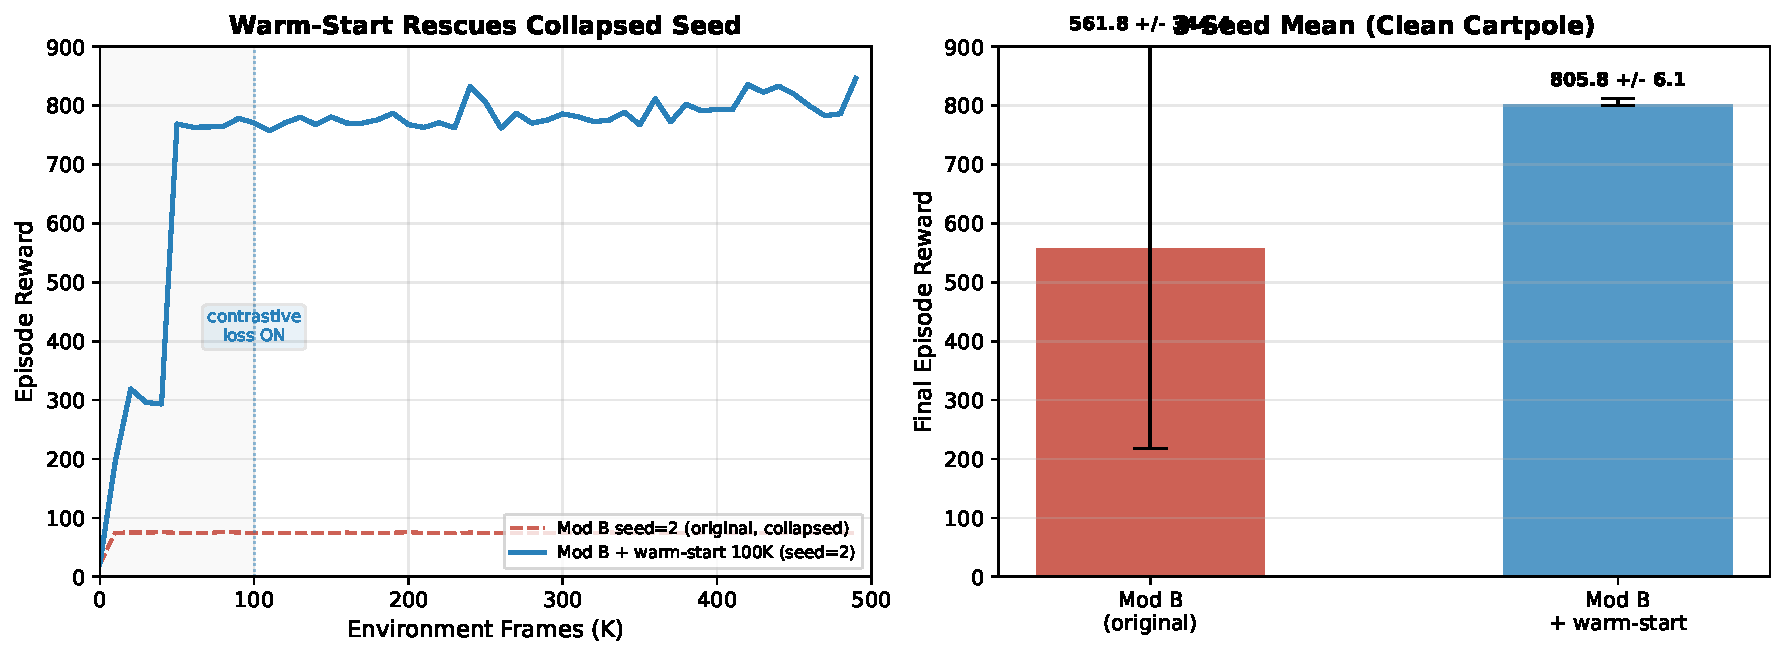
\includegraphics[width=0.95\textwidth]{figures/warmstart_simulation.pdf}
  \caption{Warm-start results for Mod~B on clean cartpole. \textbf{Left:} Learning curves for seed=2. The original Mod~B (red dashed) collapses at ${\sim}75$ for the full 500K frames. The warm-start variant (blue) delays the contrastive loss until 100K frames, allowing the Q-function to converge first, then converges to ${\sim}800$. \textbf{Right:} 3-seed final reward (seeds 1 and 3 are original Mod~B, seed 2 is warm-start). The collapsed seed is recovered from $74.8$ to $806.7$.}
  \label{fig:warmstart}
\end{figure}

\end{document}
